% Options for packages loaded elsewhere
\PassOptionsToPackage{unicode}{hyperref}
\PassOptionsToPackage{hyphens}{url}
\documentclass[
  10pt,
]{article}
\usepackage{xcolor}
\usepackage[left=2cm, right=2cm, top=2cm, bottom=2cm]{geometry}
\usepackage{amsmath,amssymb}
\setcounter{secnumdepth}{-\maxdimen} % remove section numbering
\usepackage{iftex}
\ifPDFTeX
  \usepackage[T1]{fontenc}
  \usepackage[utf8]{inputenc}
  \usepackage{textcomp} % provide euro and other symbols
\else % if luatex or xetex
  \usepackage{unicode-math} % this also loads fontspec
  \defaultfontfeatures{Scale=MatchLowercase}
  \defaultfontfeatures[\rmfamily]{Ligatures=TeX,Scale=1}
\fi
\usepackage{lmodern}
\ifPDFTeX\else
  % xetex/luatex font selection
\fi
% Use upquote if available, for straight quotes in verbatim environments
\IfFileExists{upquote.sty}{\usepackage{upquote}}{}
\IfFileExists{microtype.sty}{% use microtype if available
  \usepackage[]{microtype}
  \UseMicrotypeSet[protrusion]{basicmath} % disable protrusion for tt fonts
}{}
\makeatletter
\@ifundefined{KOMAClassName}{% if non-KOMA class
  \IfFileExists{parskip.sty}{%
    \usepackage{parskip}
  }{% else
    \setlength{\parindent}{0pt}
    \setlength{\parskip}{6pt plus 2pt minus 1pt}}
}{% if KOMA class
  \KOMAoptions{parskip=half}}
\makeatother
\usepackage{color}
\usepackage{fancyvrb}
\newcommand{\VerbBar}{|}
\newcommand{\VERB}{\Verb[commandchars=\\\{\}]}
\DefineVerbatimEnvironment{Highlighting}{Verbatim}{commandchars=\\\{\}}
% Add ',fontsize=\small' for more characters per line
\usepackage{framed}
\definecolor{shadecolor}{RGB}{248,248,248}
\newenvironment{Shaded}{\begin{snugshade}}{\end{snugshade}}
\newcommand{\AlertTok}[1]{\textcolor[rgb]{0.94,0.16,0.16}{#1}}
\newcommand{\AnnotationTok}[1]{\textcolor[rgb]{0.56,0.35,0.01}{\textbf{\textit{#1}}}}
\newcommand{\AttributeTok}[1]{\textcolor[rgb]{0.13,0.29,0.53}{#1}}
\newcommand{\BaseNTok}[1]{\textcolor[rgb]{0.00,0.00,0.81}{#1}}
\newcommand{\BuiltInTok}[1]{#1}
\newcommand{\CharTok}[1]{\textcolor[rgb]{0.31,0.60,0.02}{#1}}
\newcommand{\CommentTok}[1]{\textcolor[rgb]{0.56,0.35,0.01}{\textit{#1}}}
\newcommand{\CommentVarTok}[1]{\textcolor[rgb]{0.56,0.35,0.01}{\textbf{\textit{#1}}}}
\newcommand{\ConstantTok}[1]{\textcolor[rgb]{0.56,0.35,0.01}{#1}}
\newcommand{\ControlFlowTok}[1]{\textcolor[rgb]{0.13,0.29,0.53}{\textbf{#1}}}
\newcommand{\DataTypeTok}[1]{\textcolor[rgb]{0.13,0.29,0.53}{#1}}
\newcommand{\DecValTok}[1]{\textcolor[rgb]{0.00,0.00,0.81}{#1}}
\newcommand{\DocumentationTok}[1]{\textcolor[rgb]{0.56,0.35,0.01}{\textbf{\textit{#1}}}}
\newcommand{\ErrorTok}[1]{\textcolor[rgb]{0.64,0.00,0.00}{\textbf{#1}}}
\newcommand{\ExtensionTok}[1]{#1}
\newcommand{\FloatTok}[1]{\textcolor[rgb]{0.00,0.00,0.81}{#1}}
\newcommand{\FunctionTok}[1]{\textcolor[rgb]{0.13,0.29,0.53}{\textbf{#1}}}
\newcommand{\ImportTok}[1]{#1}
\newcommand{\InformationTok}[1]{\textcolor[rgb]{0.56,0.35,0.01}{\textbf{\textit{#1}}}}
\newcommand{\KeywordTok}[1]{\textcolor[rgb]{0.13,0.29,0.53}{\textbf{#1}}}
\newcommand{\NormalTok}[1]{#1}
\newcommand{\OperatorTok}[1]{\textcolor[rgb]{0.81,0.36,0.00}{\textbf{#1}}}
\newcommand{\OtherTok}[1]{\textcolor[rgb]{0.56,0.35,0.01}{#1}}
\newcommand{\PreprocessorTok}[1]{\textcolor[rgb]{0.56,0.35,0.01}{\textit{#1}}}
\newcommand{\RegionMarkerTok}[1]{#1}
\newcommand{\SpecialCharTok}[1]{\textcolor[rgb]{0.81,0.36,0.00}{\textbf{#1}}}
\newcommand{\SpecialStringTok}[1]{\textcolor[rgb]{0.31,0.60,0.02}{#1}}
\newcommand{\StringTok}[1]{\textcolor[rgb]{0.31,0.60,0.02}{#1}}
\newcommand{\VariableTok}[1]{\textcolor[rgb]{0.00,0.00,0.00}{#1}}
\newcommand{\VerbatimStringTok}[1]{\textcolor[rgb]{0.31,0.60,0.02}{#1}}
\newcommand{\WarningTok}[1]{\textcolor[rgb]{0.56,0.35,0.01}{\textbf{\textit{#1}}}}
\usepackage{longtable,booktabs,array}
\usepackage{calc} % for calculating minipage widths
% Correct order of tables after \paragraph or \subparagraph
\usepackage{etoolbox}
\makeatletter
\patchcmd\longtable{\par}{\if@noskipsec\mbox{}\fi\par}{}{}
\makeatother
% Allow footnotes in longtable head/foot
\IfFileExists{footnotehyper.sty}{\usepackage{footnotehyper}}{\usepackage{footnote}}
\makesavenoteenv{longtable}
\usepackage{graphicx}
\makeatletter
\newsavebox\pandoc@box
\newcommand*\pandocbounded[1]{% scales image to fit in text height/width
  \sbox\pandoc@box{#1}%
  \Gscale@div\@tempa{\textheight}{\dimexpr\ht\pandoc@box+\dp\pandoc@box\relax}%
  \Gscale@div\@tempb{\linewidth}{\wd\pandoc@box}%
  \ifdim\@tempb\p@<\@tempa\p@\let\@tempa\@tempb\fi% select the smaller of both
  \ifdim\@tempa\p@<\p@\scalebox{\@tempa}{\usebox\pandoc@box}%
  \else\usebox{\pandoc@box}%
  \fi%
}
% Set default figure placement to htbp
\def\fps@figure{htbp}
\makeatother
\setlength{\emergencystretch}{3em} % prevent overfull lines
\providecommand{\tightlist}{%
  \setlength{\itemsep}{0pt}\setlength{\parskip}{0pt}}
\usepackage{microtype}
\usepackage{fvextra}
\DefineVerbatimEnvironment{Highlighting}{Verbatim}{breaklines,commandchars=\\\{\}}
\sloppy
\usepackage{longtable}
\usepackage{fvextra}
\usepackage{bookmark}
\IfFileExists{xurl.sty}{\usepackage{xurl}}{} % add URL line breaks if available
\urlstyle{same}
\hypersetup{
  pdftitle={LOAN DATA ANALYSIS},
  pdfauthor={Wesley M. Gathua},
  hidelinks,
  pdfcreator={LaTeX via pandoc}}

\title{LOAN DATA ANALYSIS}
\author{Wesley M. Gathua}
\date{2026-04-12}

\begin{document}
\maketitle

This is my attempt to investigate the Loan Data as I try to see the
patterns and the distribution that govern this dataset.

\begin{Shaded}
\begin{Highlighting}[]
\CommentTok{\# Loading the data to R}
\NormalTok{df }\OtherTok{\textless{}{-}} \FunctionTok{read.csv}\NormalTok{(}\StringTok{"C:/Users/HP/OneDrive {-} Strathmore University/STRATH UNI/FIRST YEAR/SEMESTER III/UNITS/LINEAR MODELS/LINEAR{-}MODELS/Data/loan\_data.csv"}\NormalTok{)}

\ControlFlowTok{if}\NormalTok{ (}\FunctionTok{exists}\NormalTok{(}\StringTok{"df"}\NormalTok{)) \{}
    \FunctionTok{print}\NormalTok{(}\StringTok{"Your Loan dataset has loaded successfully!"}\NormalTok{)}
\NormalTok{\}}
\end{Highlighting}
\end{Shaded}

\begin{verbatim}
#> [1] "Your Loan dataset has loaded successfully!"
\end{verbatim}

Upon loading the dataset successfully, I proceeded to conduct some
investigations of the dataset to see what I am working with.

\begin{Shaded}
\begin{Highlighting}[]
\CommentTok{\# Checking for the numbers of rows and columns}
\FunctionTok{dim}\NormalTok{(df)}
\end{Highlighting}
\end{Shaded}

\begin{verbatim}
#> [1] 45000    14
\end{verbatim}

\begin{Shaded}
\begin{Highlighting}[]
\FunctionTok{print}\NormalTok{(}\FunctionTok{strrep}\NormalTok{(}\StringTok{"*"}\NormalTok{, }\DecValTok{50}\NormalTok{))}
\end{Highlighting}
\end{Shaded}

\begin{verbatim}
#> [1] "**************************************************"
\end{verbatim}

\begin{Shaded}
\begin{Highlighting}[]
\CommentTok{\# Checking the names of the columns}
\FunctionTok{names}\NormalTok{(df)}
\end{Highlighting}
\end{Shaded}

\begin{verbatim}
#>  [1] "person_age"                    
#>  [2] "person_gender"                 
#>  [3] "person_education"              
#>  [4] "person_income"                 
#>  [5] "person_emp_exp"                
#>  [6] "person_home_ownership"         
#>  [7] "loan_amnt"                     
#>  [8] "loan_intent"                   
#>  [9] "loan_int_rate"                 
#> [10] "loan_percent_income"           
#> [11] "cb_person_cred_hist_length"    
#> [12] "credit_score"                  
#> [13] "previous_loan_defaults_on_file"
#> [14] "loan_status"
\end{verbatim}

\begin{Shaded}
\begin{Highlighting}[]
\FunctionTok{print}\NormalTok{(}\FunctionTok{strrep}\NormalTok{(}\StringTok{"*"}\NormalTok{, }\DecValTok{50}\NormalTok{))}
\end{Highlighting}
\end{Shaded}

\begin{verbatim}
#> [1] "**************************************************"
\end{verbatim}

\begin{Shaded}
\begin{Highlighting}[]
\CommentTok{\# checking the first few rows}
\FunctionTok{View}\NormalTok{(df)}
\FunctionTok{print}\NormalTok{(}\FunctionTok{strrep}\NormalTok{(}\StringTok{"*"}\NormalTok{, }\DecValTok{50}\NormalTok{))}
\end{Highlighting}
\end{Shaded}

\begin{verbatim}
#> [1] "**************************************************"
\end{verbatim}

\begin{Shaded}
\begin{Highlighting}[]
\CommentTok{\# Checking the data type of the various columns}
\FunctionTok{str}\NormalTok{(df)}
\end{Highlighting}
\end{Shaded}

\begin{verbatim}
#> 'data.frame':    45000 obs. of  14 variables:
#>  $ person_age                    : num  22 21 25 23 24 21 26 24 24 21 ...
#>  $ person_gender                 : chr  "female" "female" "female" "female" ...
#>  $ person_education              : chr  "Master" "High School" "High School" "Bachelor" ...
#>  $ person_income                 : num  71948 12282 12438 79753 66135 ...
#>  $ person_emp_exp                : int  0 0 3 0 1 0 1 5 3 0 ...
#>  $ person_home_ownership         : chr  "RENT" "OWN" "MORTGAGE" "RENT" ...
#>  $ loan_amnt                     : num  35000 1000 5500 35000 35000 2500 35000 35000 35000 1600 ...
#>  $ loan_intent                   : chr  "PERSONAL" "EDUCATION" "MEDICAL" "MEDICAL" ...
#>  $ loan_int_rate                 : num  16 11.1 12.9 15.2 14.3 ...
#>  $ loan_percent_income           : num  0.49 0.08 0.44 0.44 0.53 0.19 0.37 0.37 0.35 0.13 ...
#>  $ cb_person_cred_hist_length    : num  3 2 3 2 4 2 3 4 2 3 ...
#>  $ credit_score                  : int  561 504 635 675 586 532 701 585 544 640 ...
#>  $ previous_loan_defaults_on_file: chr  "No" "Yes" "No" "No" ...
#>  $ loan_status                   : int  1 0 1 1 1 1 1 1 1 1 ...
\end{verbatim}

\begin{Shaded}
\begin{Highlighting}[]
\FunctionTok{print}\NormalTok{(}\FunctionTok{strrep}\NormalTok{(}\StringTok{"*"}\NormalTok{, }\DecValTok{50}\NormalTok{))}
\end{Highlighting}
\end{Shaded}

\begin{verbatim}
#> [1] "**************************************************"
\end{verbatim}

\begin{Shaded}
\begin{Highlighting}[]
\CommentTok{\# checking for null values}
\FunctionTok{colSums}\NormalTok{(}\FunctionTok{is.na}\NormalTok{(df))}
\end{Highlighting}
\end{Shaded}

\begin{verbatim}
#>                     person_age 
#>                              0 
#>                  person_gender 
#>                              0 
#>               person_education 
#>                              0 
#>                  person_income 
#>                              0 
#>                 person_emp_exp 
#>                              0 
#>          person_home_ownership 
#>                              0 
#>                      loan_amnt 
#>                              0 
#>                    loan_intent 
#>                              0 
#>                  loan_int_rate 
#>                              0 
#>            loan_percent_income 
#>                              0 
#>     cb_person_cred_hist_length 
#>                              0 
#>                   credit_score 
#>                              0 
#> previous_loan_defaults_on_file 
#>                              0 
#>                    loan_status 
#>                              0
\end{verbatim}

\begin{Shaded}
\begin{Highlighting}[]
\FunctionTok{print}\NormalTok{(}\FunctionTok{strrep}\NormalTok{(}\StringTok{"*"}\NormalTok{, }\DecValTok{50}\NormalTok{))}
\end{Highlighting}
\end{Shaded}

\begin{verbatim}
#> [1] "**************************************************"
\end{verbatim}

Upon some of the initial investigations, it was determined that there
were no null values in this dataset. There were 14 columns in this
dataset for the 45000 rows. The next step was to conduct the summary
statistics.\\

\begin{Shaded}
\begin{Highlighting}[]
\FunctionTok{summary}\NormalTok{(df)}
\end{Highlighting}
\end{Shaded}

\begin{verbatim}
#>    person_age     person_gender      person_education  
#>  Min.   : 20.00   Length:45000       Length:45000      
#>  1st Qu.: 24.00   Class :character   Class :character  
#>  Median : 26.00   Mode  :character   Mode  :character  
#>  Mean   : 27.76                                        
#>  3rd Qu.: 30.00                                        
#>  Max.   :144.00                                        
#>  person_income     person_emp_exp   person_home_ownership
#>  Min.   :   8000   Min.   :  0.00   Length:45000         
#>  1st Qu.:  47204   1st Qu.:  1.00   Class :character     
#>  Median :  67048   Median :  4.00   Mode  :character     
#>  Mean   :  80319   Mean   :  5.41                        
#>  3rd Qu.:  95789   3rd Qu.:  8.00                        
#>  Max.   :7200766   Max.   :125.00                        
#>    loan_amnt     loan_intent        loan_int_rate  
#>  Min.   :  500   Length:45000       Min.   : 5.42  
#>  1st Qu.: 5000   Class :character   1st Qu.: 8.59  
#>  Median : 8000   Mode  :character   Median :11.01  
#>  Mean   : 9583                      Mean   :11.01  
#>  3rd Qu.:12237                      3rd Qu.:12.99  
#>  Max.   :35000                      Max.   :20.00  
#>  loan_percent_income cb_person_cred_hist_length
#>  Min.   :0.0000      Min.   : 2.000            
#>  1st Qu.:0.0700      1st Qu.: 3.000            
#>  Median :0.1200      Median : 4.000            
#>  Mean   :0.1397      Mean   : 5.867            
#>  3rd Qu.:0.1900      3rd Qu.: 8.000            
#>  Max.   :0.6600      Max.   :30.000            
#>   credit_score   previous_loan_defaults_on_file
#>  Min.   :390.0   Length:45000                  
#>  1st Qu.:601.0   Class :character              
#>  Median :640.0   Mode  :character              
#>  Mean   :632.6                                 
#>  3rd Qu.:670.0                                 
#>  Max.   :850.0                                 
#>   loan_status    
#>  Min.   :0.0000  
#>  1st Qu.:0.0000  
#>  Median :0.0000  
#>  Mean   :0.2222  
#>  3rd Qu.:0.0000  
#>  Max.   :1.0000
\end{verbatim}

From the summary statistics, there was some slight skewness amongst the
columns. More pronounced skewness was seen at \emph{person\_income} and
\emph{loan\_amnt}. The means of these variables were greater than the
median. This indicated \texttt{positive\ skew}. Most of all columns
seemed to show median and mean being close to each other. Assumption of
normality would be investigated later on.\\

The next step was to establish the important features. My goal was to
see the variables that well predict the \emph{person\_income}. This was
selected to be the y(dependent) variable. In order to achieve this, the
library \texttt{finalfit} was invoked. This aided in selecting the
important features out of the remaining 13.\\

Just before this, from the \texttt{str(df)} earlier on when
investigating the data types, some variables needed to be converted from
character to categories. This is for the \texttt{finalfit} library to
actually handle all the features.\\

\begin{Shaded}
\begin{Highlighting}[]
\FunctionTok{library}\NormalTok{(dplyr)}
\NormalTok{df }\OtherTok{\textless{}{-}}\NormalTok{ df }\SpecialCharTok{|\textgreater{}}
    \FunctionTok{mutate}\NormalTok{(}\FunctionTok{across}\NormalTok{(}\FunctionTok{where}\NormalTok{(is.character), as.factor))}
\end{Highlighting}
\end{Shaded}

Now checking the important features for predicting income:\\

\begin{Shaded}
\begin{Highlighting}[]
\FunctionTok{library}\NormalTok{(dplyr)  }\CommentTok{\# goes together with finalfit}
\FunctionTok{library}\NormalTok{(finalfit)  }\CommentTok{\# main library}

\NormalTok{dependent }\OtherTok{\textless{}{-}} \StringTok{"person\_income"}
\NormalTok{explanatory }\OtherTok{\textless{}{-}} \FunctionTok{names}\NormalTok{(df)[}\FunctionTok{names}\NormalTok{(df) }\SpecialCharTok{!=}\NormalTok{ dependent]  }\CommentTok{\# selecting all other columns}

\NormalTok{results }\OtherTok{\textless{}{-}}\NormalTok{ df }\SpecialCharTok{|\textgreater{}}
    \FunctionTok{finalfit}\NormalTok{(dependent, explanatory)  }\CommentTok{\# passing the data into the finalfit function}
\FunctionTok{View}\NormalTok{(results)}
\NormalTok{results }\SpecialCharTok{|\textgreater{}}
\NormalTok{    knitr}\SpecialCharTok{::}\FunctionTok{kable}\NormalTok{(}\AttributeTok{caption =} \StringTok{"Multivariable Linear Regression of a person\textquotesingle{}s income"}\NormalTok{)  }\CommentTok{\# table for R markdown}
\end{Highlighting}
\end{Shaded}

\begin{longtable}[]{@{}
  >{\raggedright\arraybackslash}p{(\linewidth - 12\tabcolsep) * \real{0.0170}}
  >{\raggedright\arraybackslash}p{(\linewidth - 12\tabcolsep) * \real{0.1761}}
  >{\raggedright\arraybackslash}p{(\linewidth - 12\tabcolsep) * \real{0.1023}}
  >{\raggedright\arraybackslash}p{(\linewidth - 12\tabcolsep) * \real{0.0568}}
  >{\raggedright\arraybackslash}p{(\linewidth - 12\tabcolsep) * \real{0.1136}}
  >{\raggedright\arraybackslash}p{(\linewidth - 12\tabcolsep) * \real{0.2670}}
  >{\raggedright\arraybackslash}p{(\linewidth - 12\tabcolsep) * \real{0.2670}}@{}}
\caption{Multivariable Linear Regression of a person's
income}\tabularnewline
\toprule\noalign{}
\begin{minipage}[b]{\linewidth}\raggedright
\end{minipage} & \begin{minipage}[b]{\linewidth}\raggedright
Dependent: person\_income
\end{minipage} & \begin{minipage}[b]{\linewidth}\raggedright
\end{minipage} & \begin{minipage}[b]{\linewidth}\raggedright
unit
\end{minipage} & \begin{minipage}[b]{\linewidth}\raggedright
value
\end{minipage} & \begin{minipage}[b]{\linewidth}\raggedright
Coefficient (univariable)
\end{minipage} & \begin{minipage}[b]{\linewidth}\raggedright
Coefficient (multivariable)
\end{minipage} \\
\midrule\noalign{}
\endfirsthead
\toprule\noalign{}
\begin{minipage}[b]{\linewidth}\raggedright
\end{minipage} & \begin{minipage}[b]{\linewidth}\raggedright
Dependent: person\_income
\end{minipage} & \begin{minipage}[b]{\linewidth}\raggedright
\end{minipage} & \begin{minipage}[b]{\linewidth}\raggedright
unit
\end{minipage} & \begin{minipage}[b]{\linewidth}\raggedright
value
\end{minipage} & \begin{minipage}[b]{\linewidth}\raggedright
Coefficient (univariable)
\end{minipage} & \begin{minipage}[b]{\linewidth}\raggedright
Coefficient (multivariable)
\end{minipage} \\
\midrule\noalign{}
\endhead
\bottomrule\noalign{}
\endlastfoot
14 & person\_age & {[}20.0,144.0{]} & Mean (sd) & 80319.1 (80422.5) &
2576.90 (2456.31 to 2697.50, p\textless0.001) & 3002.63 (2618.85 to
3386.40, p\textless0.001) \\
21 & person\_gender & female & Mean (sd) & 79410.9 (77759.5) & - & - \\
22 & & male & Mean (sd) & 81056.0 (82514.6) & 1645.13 (150.94 to
3139.32, p=0.031) & 167.76 (-1075.20 to 1410.72, p=0.791) \\
15 & person\_education & Associate & Mean (sd) & 80641.6 (90097.7) & - &
- \\
16 & & Bachelor & Mean (sd) & 79703.3 (73348.2) & -938.30 (-2918.21 to
1041.60, p=0.353) & 766.33 (-888.88 to 2421.55, p=0.364) \\
17 & & Doctorate & Mean (sd) & 87234.5 (87156.3) & 6592.92 (106.35 to
13079.49, p=0.046) & -5083.38 (-10521.81 to 355.05, p=0.067) \\
18 & & High School & Mean (sd) & 80224.6 (88693.8) & -417.03 (-2451.98
to 1617.93, p=0.688) & 335.30 (-1362.70 to 2033.29, p=0.699) \\
19 & & Master & Mean (sd) & 80491.9 (56673.3) & -149.70 (-2521.47 to
2222.07, p=0.902) & 46.52 (-1942.62 to 2035.65, p=0.963) \\
20 & person\_emp\_exp & {[}0.0,125.0{]} & Mean (sd) & 80319.1 (80422.5)
& 2466.80 (2346.39 to 2587.22, p\textless0.001) & 649.70 (307.35 to
992.04, p\textless0.001) \\
23 & person\_home\_ownership & MORTGAGE & Mean (sd) & 101569.3
(108180.6) & - & - \\
24 & & OTHER & Mean (sd) & 91480.1 (94488.6) & -10089.24 (-24345.40 to
4166.92, p=0.165) & 5068.91 (-7098.46 to 17236.28, p=0.414) \\
25 & & OWN & Mean (sd) & 68423.4 (60439.3) & -33145.90 (-36193.07 to
-30098.73, p\textless0.001) & -2051.01 (-4721.92 to 619.90, p=0.132) \\
26 & & RENT & Mean (sd) & 65001.1 (45525.0) & -36568.16 (-38080.11 to
-35056.22, p\textless0.001) & -8974.47 (-10366.86 to -7582.08,
p\textless0.001) \\
3 & loan\_amnt & {[}500.0,35000.0{]} & Mean (sd) & 80319.1 (80422.5) &
3.09 (2.97 to 3.20, p\textless0.001) & 7.17 (7.04 to 7.30,
p\textless0.001) \\
5 & loan\_intent & DEBTCONSOLIDATION & Mean (sd) & 80608.2 (63435.9) & -
& - \\
6 & & EDUCATION & Mean (sd) & 77765.0 (52791.0) & -2843.19 (-5327.73 to
-358.65, p=0.025) & 277.12 (-1810.51 to 2364.75, p=0.795) \\
7 & & HOMEIMPROVEMENT & Mean (sd) & 89148.7 (58538.4) & 8540.53 (5600.21
to 11480.85, p\textless0.001) & -2404.06 (-4866.16 to 58.04, p=0.056) \\
8 & & MEDICAL & Mean (sd) & 73414.9 (62636.0) & -7193.35 (-9716.14 to
-4670.55, p\textless0.001) & -1998.58 (-4106.05 to 108.89, p=0.063) \\
9 & & PERSONAL & Mean (sd) & 83030.9 (108157.3) & 2422.69 (-174.74 to
5020.13, p=0.068) & 1346.51 (-827.49 to 3520.51, p=0.225) \\
10 & & VENTURE & Mean (sd) & 82572.0 (111733.7) & 1963.75 (-612.03 to
4539.53, p=0.135) & 2574.66 (400.06 to 4749.26, p=0.020) \\
4 & loan\_int\_rate & {[}5.4,20.0{]} & Mean (sd) & 80319.1 (80422.5) &
40.76 (-208.70 to 290.22, p=0.749) & -513.11 (-737.00 to -289.22,
p\textless0.001) \\
11 & loan\_percent\_income & {[}0.0,0.7{]} & Mean (sd) & 80319.1
(80422.5) & -215945.01 (-224228.55 to -207661.48, p\textless0.001) &
-525819.20 (-535870.55 to -515767.86, p\textless0.001) \\
1 & cb\_person\_cred\_hist\_length & {[}2.0,30.0{]} & Mean (sd) &
80319.1 (80422.5) & 2576.94 (2386.90 to 2766.99, p\textless0.001) &
-3144.27 (-3458.74 to -2829.79, p\textless0.001) \\
2 & credit\_score & {[}390.0,850.0{]} & Mean (sd) & 80319.1 (80422.5) &
57.27 (42.55 to 72.00, p\textless0.001) & -2.56 (-15.63 to 10.52,
p=0.702) \\
27 & previous\_loan\_defaults\_on\_file & No & Mean (sd) & 75295.2
(92023.6) & - & - \\
28 & & Yes & Mean (sd) & 85185.6 (66947.9) & 9890.41 (8406.87 to
11373.95, p\textless0.001) & -762.71 (-2272.91 to 747.50, p=0.322) \\
12 & loan\_status & 0 & Mean (sd) & 86157.0 (87035.2) & - & - \\
13 & & 1 & Mean (sd) & 59886.1 (45338.3) & -26270.94 (-28041.75 to
-24500.13, p\textless0.001) & 8922.76 (6887.43 to 10958.08,
p\textless0.001) \\
\end{longtable}

\begin{Shaded}
\begin{Highlighting}[]
\NormalTok{results\_summary }\OtherTok{\textless{}{-}}\NormalTok{ df }\SpecialCharTok{|\textgreater{}}
    \FunctionTok{summary\_factorlist}\NormalTok{(dependent, explanatory)  }\CommentTok{\# summary of the finalfit research}
\NormalTok{results\_summary }\SpecialCharTok{|\textgreater{}}
\NormalTok{    knitr}\SpecialCharTok{::}\FunctionTok{kable}\NormalTok{(}\AttributeTok{caption =} \StringTok{"Summary Factor List"}\NormalTok{)}
\end{Highlighting}
\end{Shaded}

\begin{longtable}[]{@{}
  >{\raggedright\arraybackslash}p{(\linewidth - 6\tabcolsep) * \real{0.3924}}
  >{\raggedright\arraybackslash}p{(\linewidth - 6\tabcolsep) * \real{0.2278}}
  >{\raggedright\arraybackslash}p{(\linewidth - 6\tabcolsep) * \real{0.1266}}
  >{\raggedright\arraybackslash}p{(\linewidth - 6\tabcolsep) * \real{0.2532}}@{}}
\caption{Summary Factor List}\tabularnewline
\toprule\noalign{}
\begin{minipage}[b]{\linewidth}\raggedright
label
\end{minipage} & \begin{minipage}[b]{\linewidth}\raggedright
levels
\end{minipage} & \begin{minipage}[b]{\linewidth}\raggedright
unit
\end{minipage} & \begin{minipage}[b]{\linewidth}\raggedright
value
\end{minipage} \\
\midrule\noalign{}
\endfirsthead
\toprule\noalign{}
\begin{minipage}[b]{\linewidth}\raggedright
label
\end{minipage} & \begin{minipage}[b]{\linewidth}\raggedright
levels
\end{minipage} & \begin{minipage}[b]{\linewidth}\raggedright
unit
\end{minipage} & \begin{minipage}[b]{\linewidth}\raggedright
value
\end{minipage} \\
\midrule\noalign{}
\endhead
\bottomrule\noalign{}
\endlastfoot
person\_age & {[}20.0,144.0{]} & Mean (sd) & 80319.1 (80422.5) \\
person\_gender & female & Mean (sd) & 79410.9 (77759.5) \\
& male & Mean (sd) & 81056.0 (82514.6) \\
person\_education & Associate & Mean (sd) & 80641.6 (90097.7) \\
& Bachelor & Mean (sd) & 79703.3 (73348.2) \\
& Doctorate & Mean (sd) & 87234.5 (87156.3) \\
& High School & Mean (sd) & 80224.6 (88693.8) \\
& Master & Mean (sd) & 80491.9 (56673.3) \\
person\_emp\_exp & {[}0.0,125.0{]} & Mean (sd) & 80319.1 (80422.5) \\
person\_home\_ownership & MORTGAGE & Mean (sd) & 101569.3 (108180.6) \\
& OTHER & Mean (sd) & 91480.1 (94488.6) \\
& OWN & Mean (sd) & 68423.4 (60439.3) \\
& RENT & Mean (sd) & 65001.1 (45525.0) \\
loan\_amnt & {[}500.0,35000.0{]} & Mean (sd) & 80319.1 (80422.5) \\
loan\_intent & DEBTCONSOLIDATION & Mean (sd) & 80608.2 (63435.9) \\
& EDUCATION & Mean (sd) & 77765.0 (52791.0) \\
& HOMEIMPROVEMENT & Mean (sd) & 89148.7 (58538.4) \\
& MEDICAL & Mean (sd) & 73414.9 (62636.0) \\
& PERSONAL & Mean (sd) & 83030.9 (108157.3) \\
& VENTURE & Mean (sd) & 82572.0 (111733.7) \\
loan\_int\_rate & {[}5.4,20.0{]} & Mean (sd) & 80319.1 (80422.5) \\
loan\_percent\_income & {[}0.0,0.7{]} & Mean (sd) & 80319.1 (80422.5) \\
cb\_person\_cred\_hist\_length & {[}2.0,30.0{]} & Mean (sd) & 80319.1
(80422.5) \\
credit\_score & {[}390.0,850.0{]} & Mean (sd) & 80319.1 (80422.5) \\
previous\_loan\_defaults\_on\_file & No & Mean (sd) & 75295.2
(92023.6) \\
& Yes & Mean (sd) & 85185.6 (66947.9) \\
loan\_status & 0 & Mean (sd) & 86157.0 (87035.2) \\
& 1 & Mean (sd) & 59886.1 (45338.3) \\
\end{longtable}

The above tables provided a deeper understanding of the
\texttt{loans\ dataset}.\\
The following was deduced:\\
\textbf{(i) Summary Factor List Table}\\

\begin{enumerate}
\def\labelenumi{\alph{enumi})}
\item
  Some of the columns exhibited some outliers. The \texttt{person\_age}
  column had a minimum age of 20 and a maximum of \emph{144}. The
  \texttt{person\_emp\_exp} column had a minimum experience of 0 years
  and a maximum of \emph{125} years. These outliers would greatly affect
  their respective means as well us lead to a violation of linearity
  assumptions. They would be taken care off in subsequent sections.\\
\item
  From the various means (averages) one is able to deduce which
  categories had more income as compared to the rest. For instance
  looking at the \texttt{person\_education}, it was seen that people who
  have a Doctorate earn highly (\$87234.5) compared to the remaining
  levels of education such as Bachelor graduates (\$79703.3).
\end{enumerate}

\textbf{(ii) Multivariable Linear Regression of a person's income}\\

This is where much of the information was discovered.\\

\begin{enumerate}
\def\labelenumi{\alph{enumi})}
\item
  Some of the columns were seen to be significant under the univariate
  coefficient column as they became less significant in the multivariate
  coefficient column. Looking at \texttt{person\_gender}, under
  univariate statistics, it was seen that it was a significant column
  with its p-value at 0.031. The multivariate coefficient was 0.791.
  This meant that it was only significant being the \textbf{only}
  predictor but when all other variables are included and held constant,
  its effect reduces. It was not a significant predictor of a person's
  income.\\
\item
  Similar to the \texttt{Summary\ Factor\ List} table, it was evident
  that different categories had more income as compared to the rest.
  Observing \texttt{person\_home\_ownership} variable, \texttt{mortgage}
  being selected as the base, it was evident that mortgage owners had
  the highest income. The coefficients of both univariate and
  multivariate analysis exhibited the rest having negative values
  indicating that they were below the baseline \texttt{mortgage}.
  Looking at the statistical significance under univariate, owning a
  house (\texttt{own}) and renting (\texttt{rent}) had a low p-value
  (\(< 0.05\)) indicating that they greatly affected
  \texttt{person\_income}.\\
\end{enumerate}

The table below presents the significant variables as per the p-values
from the univariate analysis. This is because some of these variables
could be having some correlation with other variables making the
p-values of their multivariate analysis be high. This was to prevent
deletion of variables pre-maturely.\\

\begin{Shaded}
\begin{Highlighting}[]
\NormalTok{variables }\OtherTok{\textless{}{-}} \FunctionTok{c}\NormalTok{(}\StringTok{"person\_age"}\NormalTok{, }\StringTok{"person\_gender"}\NormalTok{, }\StringTok{"person\_education"}\NormalTok{,}
    \StringTok{"person\_emp\_exp"}\NormalTok{, }\StringTok{"person\_home\_ownership"}\NormalTok{, }\StringTok{"loan\_amnt"}\NormalTok{, }\StringTok{"loan\_intent"}\NormalTok{,}
    \StringTok{"loan\_percent\_income"}\NormalTok{, }\StringTok{"cb\_person\_cred\_hist\_length"}\NormalTok{, }\StringTok{"credit\_score"}\NormalTok{,}
    \StringTok{"previous\_loan\_defaults\_on\_file"}\NormalTok{, }\StringTok{"loan\_status"}\NormalTok{)}
\NormalTok{univariate\_p\_values }\OtherTok{\textless{}{-}} \FunctionTok{c}\NormalTok{(}\StringTok{"p\textless{}0.001"}\NormalTok{, }\StringTok{"p=0.031"}\NormalTok{, }\StringTok{"p=0.046 (Doctorate)"}\NormalTok{,}
    \StringTok{"p\textless{}0.001"}\NormalTok{, }\StringTok{"p\textless{}0.001 (OWN \& RENT)"}\NormalTok{, }\StringTok{"p\textless{}0.001"}\NormalTok{, }\StringTok{"p\textless{}0.001"}\NormalTok{,}
    \StringTok{"p\textless{}0.001"}\NormalTok{, }\StringTok{"p\textless{}0.001"}\NormalTok{, }\StringTok{"p\textless{}0.001"}\NormalTok{, }\StringTok{"p\textless{}0.001"}\NormalTok{, }\StringTok{"p\textless{}0.001"}\NormalTok{)}

\NormalTok{significance\_table }\OtherTok{\textless{}{-}} \FunctionTok{data.frame}\NormalTok{(}\AttributeTok{Variable =}\NormalTok{ variables, }\AttributeTok{Univariate\_p\_value =}\NormalTok{ univariate\_p\_values)}

\FunctionTok{print}\NormalTok{(significance\_table)}
\end{Highlighting}
\end{Shaded}

\begin{verbatim}
#>                          Variable   Univariate_p_value
#> 1                      person_age              p<0.001
#> 2                   person_gender              p=0.031
#> 3                person_education  p=0.046 (Doctorate)
#> 4                  person_emp_exp              p<0.001
#> 5           person_home_ownership p<0.001 (OWN & RENT)
#> 6                       loan_amnt              p<0.001
#> 7                     loan_intent              p<0.001
#> 8             loan_percent_income              p<0.001
#> 9      cb_person_cred_hist_length              p<0.001
#> 10                   credit_score              p<0.001
#> 11 previous_loan_defaults_on_file              p<0.001
#> 12                    loan_status              p<0.001
\end{verbatim}

The next logical step was to build a linear regression model. This was
done before checking model assumptions. This is because the assumptions
are based on the residuals. The mathematical formula for getting the
residuals is:\\

\(e = Y - \hat{Y}\), where \(\hat{Y}\) is the predicted value.\\

This is is why the next step was to get the predicted value.\\

\begin{Shaded}
\begin{Highlighting}[]
\NormalTok{initial\_model }\OtherTok{\textless{}{-}} \FunctionTok{lm}\NormalTok{(person\_income }\SpecialCharTok{\textasciitilde{}}\NormalTok{ person\_age }\SpecialCharTok{+}\NormalTok{ person\_gender }\SpecialCharTok{+}
\NormalTok{    person\_education }\SpecialCharTok{+}\NormalTok{ person\_emp\_exp }\SpecialCharTok{+}\NormalTok{ person\_home\_ownership }\SpecialCharTok{+}
\NormalTok{    loan\_amnt }\SpecialCharTok{+}\NormalTok{ loan\_intent }\SpecialCharTok{+}\NormalTok{ loan\_percent\_income }\SpecialCharTok{+}\NormalTok{ cb\_person\_cred\_hist\_length }\SpecialCharTok{+}
\NormalTok{    credit\_score }\SpecialCharTok{+}\NormalTok{ previous\_loan\_defaults\_on\_file }\SpecialCharTok{+}\NormalTok{ loan\_status,}
    \AttributeTok{data =}\NormalTok{ df)}

\FunctionTok{summary}\NormalTok{(initial\_model)}
\end{Highlighting}
\end{Shaded}

\begin{verbatim}
#> 
#> Call:
#> lm(formula = person_income ~ person_age + person_gender + person_education + 
#>     person_emp_exp + person_home_ownership + loan_amnt + loan_intent + 
#>     loan_percent_income + cb_person_cred_hist_length + credit_score + 
#>     previous_loan_defaults_on_file + loan_status, data = df)
#> 
#> Residuals:
#>     Min      1Q  Median      3Q     Max 
#> -374050  -17501   -5209    8262 6709994 
#> 
#> Coefficients:
#>                                     Estimate Std. Error
#> (Intercept)                        2.159e+04  6.154e+03
#> person_age                         3.018e+03  1.958e+02
#> person_gendermale                  1.628e+02  6.343e+02
#> person_educationBachelor           7.437e+02  8.447e+02
#> person_educationDoctorate         -5.092e+03  2.775e+03
#> person_educationHigh School        3.246e+02  8.665e+02
#> person_educationMaster             4.016e+01  1.015e+03
#> person_emp_exp                     6.373e+02  1.747e+02
#> person_home_ownershipOTHER         4.528e+03  6.208e+03
#> person_home_ownershipOWN          -2.403e+03  1.361e+03
#> person_home_ownershipRENT         -9.305e+03  7.067e+02
#> loan_amnt                          7.120e+00  6.603e-02
#> loan_intentEDUCATION               1.800e+02  1.065e+03
#> loan_intentHOMEIMPROVEMENT        -2.500e+03  1.256e+03
#> loan_intentMEDICAL                -2.060e+03  1.075e+03
#> loan_intentPERSONAL                1.257e+03  1.109e+03
#> loan_intentVENTURE                 2.448e+03  1.109e+03
#> loan_percent_income               -5.231e+05  5.095e+03
#> cb_person_cred_hist_length        -3.153e+03  1.605e+02
#> credit_score                      -2.835e+00  6.671e+00
#> previous_loan_defaults_on_fileYes -7.695e+02  7.707e+02
#> loan_status                        7.638e+03  9.984e+02
#>                                    t value Pr(>|t|)    
#> (Intercept)                          3.508 0.000452 ***
#> person_age                          15.411  < 2e-16 ***
#> person_gendermale                    0.257 0.797498    
#> person_educationBachelor             0.881 0.378585    
#> person_educationDoctorate           -1.835 0.066566 .  
#> person_educationHigh School          0.375 0.707986    
#> person_educationMaster               0.040 0.968440    
#> person_emp_exp                       3.648 0.000264 ***
#> person_home_ownershipOTHER           0.729 0.465773    
#> person_home_ownershipOWN            -1.766 0.077391 .  
#> person_home_ownershipRENT          -13.165  < 2e-16 ***
#> loan_amnt                          107.829  < 2e-16 ***
#> loan_intentEDUCATION                 0.169 0.865765    
#> loan_intentHOMEIMPROVEMENT          -1.990 0.046603 *  
#> loan_intentMEDICAL                  -1.915 0.055447 .  
#> loan_intentPERSONAL                  1.133 0.257029    
#> loan_intentVENTURE                   2.207 0.027348 *  
#> loan_percent_income               -102.685  < 2e-16 ***
#> cb_person_cred_hist_length         -19.648  < 2e-16 ***
#> credit_score                        -0.425 0.670856    
#> previous_loan_defaults_on_fileYes   -0.998 0.318076    
#> loan_status                          7.649 2.06e-14 ***
#> ---
#> Signif. codes:  
#> 0 '***' 0.001 '**' 0.01 '*' 0.05 '.' 0.1 ' ' 1
#> 
#> Residual standard error: 66890 on 44978 degrees of freedom
#> Multiple R-squared:  0.3085, Adjusted R-squared:  0.3082 
#> F-statistic: 955.7 on 21 and 44978 DF,  p-value: < 2.2e-16
\end{verbatim}

9 variables were significant as their p-values was \textless{} 0.05.\\
The subsequent step was to investigate if the assumptions of linearity
were violated.\\

\begin{Shaded}
\begin{Highlighting}[]
\FunctionTok{plot}\NormalTok{(initial\_model)}
\end{Highlighting}
\end{Shaded}

\begin{center}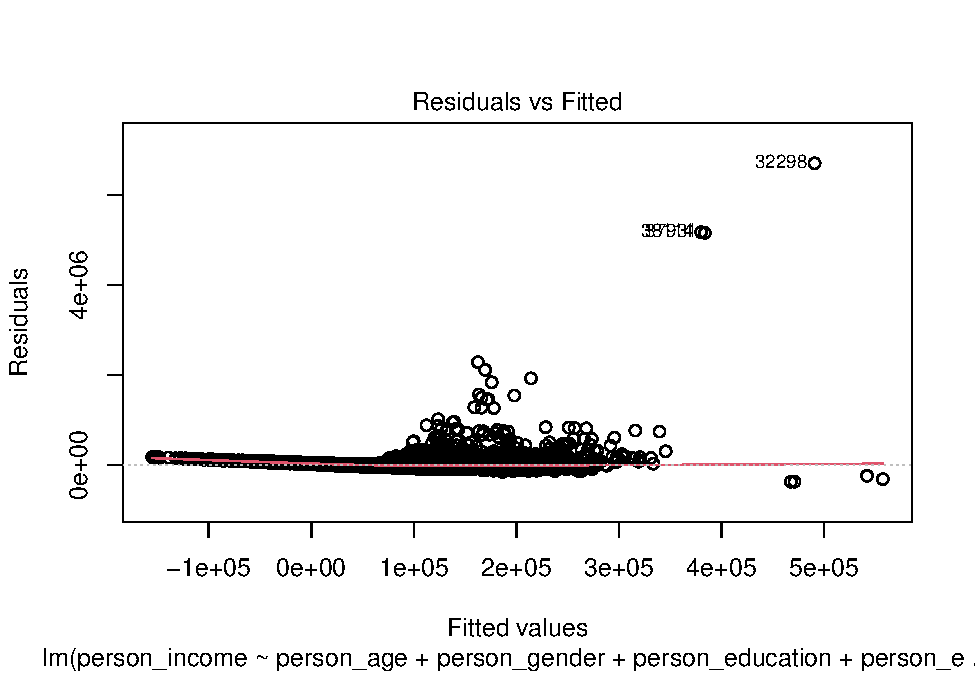
\includegraphics{Loan_data_markdown_files/figure-latex/linearity assumptions check-1} \end{center}

\begin{center}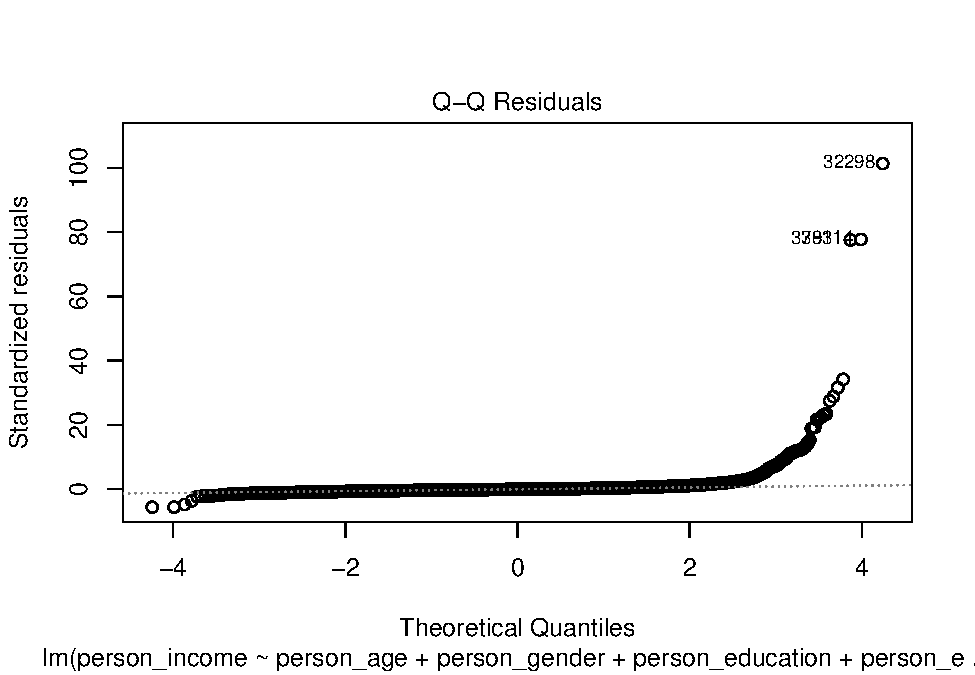
\includegraphics{Loan_data_markdown_files/figure-latex/linearity assumptions check-2} \end{center}

\begin{center}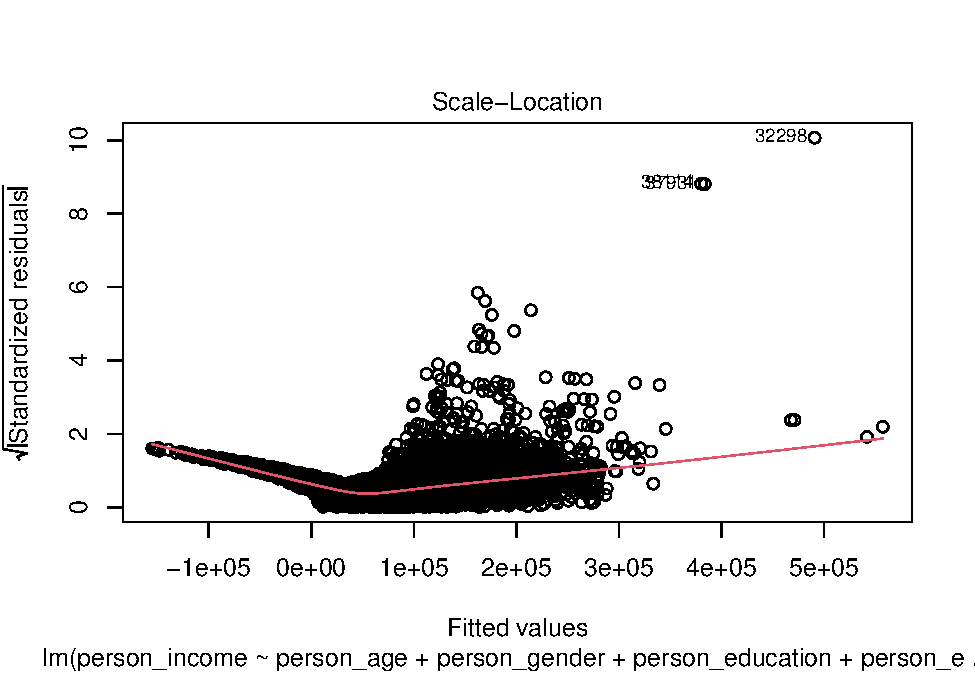
\includegraphics{Loan_data_markdown_files/figure-latex/linearity assumptions check-3} \end{center}

\begin{center}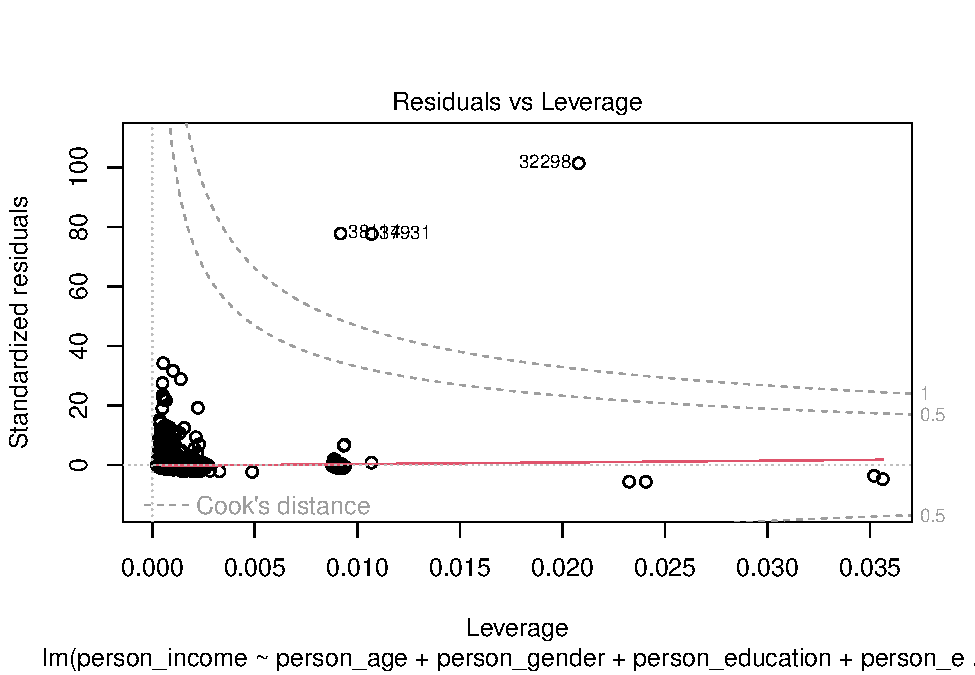
\includegraphics{Loan_data_markdown_files/figure-latex/linearity assumptions check-4} \end{center}

\textbf{1. Residuals vs Fitted Plot}\\

The data points begin being well concentrated on the red-dashed line as
they deviate from it going right. This shows the
\texttt{violation\ of\ homoskedasticity}. The variance tends to
increase.\\
The red-dashed line is relatively flat. This indicates that there was
\texttt{no\ violation\ of\ the\ linearity\ assumption}.\\

\textbf{2. Q-Q Residuals}\\

The data points are relatively on the dashed line but curve upwards as
you move to the right. This shows a \texttt{violation\ of\ normality} as
there is a positive skew.\\

\textbf{3. Scale-Location}\\

This backs up our earlier statement on the
\texttt{violation\ of\ homoskedasticity}. The red-dashed line is curved
upwards indicating heteroskedasticity.\\

\textbf{4. Residuals vs Fitted}\\

This shows that there were outliers in the dataset as they are well
outside the cook's distance.\\

Initially, we discovered some `spurious' data in the sense that we saw a
person's age to be 144 and a person who had an experience of 125 years.
This were removed (as shown below) to prevent having unreliable
results.\\

\begin{Shaded}
\begin{Highlighting}[]
\NormalTok{df\_clean }\OtherTok{\textless{}{-}}\NormalTok{ df }\SpecialCharTok{|\textgreater{}}
    \FunctionTok{filter}\NormalTok{(person\_age }\SpecialCharTok{\textless{}} \DecValTok{100}\NormalTok{, person\_emp\_exp }\SpecialCharTok{\textless{}} \DecValTok{70}\NormalTok{)}

\CommentTok{\# Checking number of rows that were deleted}
\FunctionTok{nrow}\NormalTok{(df) }\SpecialCharTok{{-}} \FunctionTok{nrow}\NormalTok{(df\_clean)}
\end{Highlighting}
\end{Shaded}

\begin{verbatim}
#> [1] 8
\end{verbatim}

8 rows were omitted.\\
We proceeded to conduct a log transformation of the dependent variable
\texttt{person\_income}.\\

\begin{Shaded}
\begin{Highlighting}[]
\NormalTok{log\_model }\OtherTok{\textless{}{-}} \FunctionTok{lm}\NormalTok{(}\FunctionTok{log}\NormalTok{(person\_income) }\SpecialCharTok{\textasciitilde{}}\NormalTok{ person\_age }\SpecialCharTok{+}\NormalTok{ person\_gender }\SpecialCharTok{+}
\NormalTok{    person\_education }\SpecialCharTok{+}\NormalTok{ person\_emp\_exp }\SpecialCharTok{+}\NormalTok{ person\_home\_ownership }\SpecialCharTok{+}
\NormalTok{    loan\_amnt }\SpecialCharTok{+}\NormalTok{ loan\_intent }\SpecialCharTok{+}\NormalTok{ loan\_percent\_income }\SpecialCharTok{+}\NormalTok{ cb\_person\_cred\_hist\_length }\SpecialCharTok{+}
\NormalTok{    credit\_score }\SpecialCharTok{+}\NormalTok{ previous\_loan\_defaults\_on\_file }\SpecialCharTok{+}\NormalTok{ loan\_status,}
    \AttributeTok{data =}\NormalTok{ df\_clean)}

\FunctionTok{summary}\NormalTok{(log\_model)}
\end{Highlighting}
\end{Shaded}

\begin{verbatim}
#> 
#> Call:
#> lm(formula = log(person_income) ~ person_age + person_gender + 
#>     person_education + person_emp_exp + person_home_ownership + 
#>     loan_amnt + loan_intent + loan_percent_income + cb_person_cred_hist_length + 
#>     credit_score + previous_loan_defaults_on_file + loan_status, 
#>     data = df_clean)
#> 
#> Residuals:
#>     Min      1Q  Median      3Q     Max 
#> -1.7402 -0.1222  0.0049  0.1189  3.2278 
#> 
#> Coefficients:
#>                                     Estimate Std. Error
#> (Intercept)                        1.107e+01  2.485e-02
#> person_age                         4.426e-03  7.995e-04
#> person_gendermale                  2.000e-05  2.543e-03
#> person_educationBachelor           6.682e-03  3.386e-03
#> person_educationDoctorate         -3.812e-05  1.113e-02
#> person_educationHigh School       -1.159e-03  3.474e-03
#> person_educationMaster             4.037e-03  4.069e-03
#> person_emp_exp                    -1.806e-03  7.009e-04
#> person_home_ownershipOTHER         3.568e-04  2.489e-02
#> person_home_ownershipOWN          -1.109e-01  5.455e-03
#> person_home_ownershipRENT         -1.046e-01  2.833e-03
#> loan_amnt                          8.276e-05  2.647e-07
#> loan_intentEDUCATION              -6.980e-03  4.270e-03
#> loan_intentHOMEIMPROVEMENT         1.173e-02  5.036e-03
#> loan_intentMEDICAL                -2.420e-02  4.311e-03
#> loan_intentPERSONAL               -1.697e-03  4.447e-03
#> loan_intentVENTURE                -3.536e-03  4.448e-03
#> loan_percent_income               -5.698e+00  2.043e-02
#> cb_person_cred_hist_length         5.775e-04  6.843e-04
#> credit_score                       1.257e-05  2.675e-05
#> previous_loan_defaults_on_fileYes -1.594e-03  3.090e-03
#> loan_status                       -2.889e-02  4.003e-03
#>                                    t value Pr(>|t|)    
#> (Intercept)                        445.600  < 2e-16 ***
#> person_age                           5.536 3.11e-08 ***
#> person_gendermale                    0.008  0.99372    
#> person_educationBachelor             1.973  0.04848 *  
#> person_educationDoctorate           -0.003  0.99727    
#> person_educationHigh School         -0.334  0.73861    
#> person_educationMaster               0.992  0.32118    
#> person_emp_exp                      -2.577  0.00997 ** 
#> person_home_ownershipOTHER           0.014  0.98856    
#> person_home_ownershipOWN           -20.323  < 2e-16 ***
#> person_home_ownershipRENT          -36.921  < 2e-16 ***
#> loan_amnt                          312.600  < 2e-16 ***
#> loan_intentEDUCATION                -1.634  0.10217    
#> loan_intentHOMEIMPROVEMENT           2.330  0.01983 *  
#> loan_intentMEDICAL                  -5.615 1.98e-08 ***
#> loan_intentPERSONAL                 -0.382  0.70272    
#> loan_intentVENTURE                  -0.795  0.42659    
#> loan_percent_income               -278.976  < 2e-16 ***
#> cb_person_cred_hist_length           0.844  0.39867    
#> credit_score                         0.470  0.63840    
#> previous_loan_defaults_on_fileYes   -0.516  0.60589    
#> loan_status                         -7.219 5.32e-13 ***
#> ---
#> Signif. codes:  
#> 0 '***' 0.001 '**' 0.01 '*' 0.05 '.' 0.1 ' ' 1
#> 
#> Residual standard error: 0.2681 on 44970 degrees of freedom
#> Multiple R-squared:  0.7677, Adjusted R-squared:  0.7676 
#> F-statistic:  7079 on 21 and 44970 DF,  p-value: < 2.2e-16
\end{verbatim}

Both the Multiple and Adjusted R-Squared doubled. Initially, the model
could only explain 30.85\% of variation but upon log transformation of
our dependent variable and cleaning our data, our model explains 76.77\%
of the variation. Approximately 30\% of the variation are explained by
other factors not in the model. The next step was to conduct stepwise
selection. This is to provide the optimum model with the most suitable
variables.\\

\begin{Shaded}
\begin{Highlighting}[]
\NormalTok{optimum\_model }\OtherTok{\textless{}{-}} \FunctionTok{step}\NormalTok{(log\_model, }\AttributeTok{direction =} \StringTok{"both"}\NormalTok{)}
\end{Highlighting}
\end{Shaded}

\begin{verbatim}
#> Start:  AIC=-118418.9
#> log(person_income) ~ person_age + person_gender + person_education + 
#>     person_emp_exp + person_home_ownership + loan_amnt + loan_intent + 
#>     loan_percent_income + cb_person_cred_hist_length + credit_score + 
#>     previous_loan_defaults_on_file + loan_status
#> 
#>                                  Df Sum of Sq     RSS
#> - person_gender                   1       0.0  3233.3
#> - credit_score                    1       0.0  3233.3
#> - previous_loan_defaults_on_file  1       0.0  3233.3
#> - person_education                4       0.5  3233.8
#> - cb_person_cred_hist_length      1       0.1  3233.4
#> <none>                                         3233.3
#> - person_emp_exp                  1       0.5  3233.8
#> - person_age                      1       2.2  3235.5
#> - loan_status                     1       3.7  3237.1
#> - loan_intent                     5       4.7  3238.0
#> - person_home_ownership           3     105.3  3338.7
#> - loan_percent_income             1    5595.7  8829.1
#> - loan_amnt                       1    7025.9 10259.2
#>                                      AIC
#> - person_gender                  -118421
#> - credit_score                   -118421
#> - previous_loan_defaults_on_file -118421
#> - person_education               -118420
#> - cb_person_cred_hist_length     -118420
#> <none>                           -118419
#> - person_emp_exp                 -118414
#> - person_age                     -118390
#> - loan_status                    -118369
#> - loan_intent                    -118363
#> - person_home_ownership          -116982
#> - loan_percent_income             -73225
#> - loan_amnt                       -66470
#> 
#> Step:  AIC=-118420.9
#> log(person_income) ~ person_age + person_education + person_emp_exp + 
#>     person_home_ownership + loan_amnt + loan_intent + loan_percent_income + 
#>     cb_person_cred_hist_length + credit_score + previous_loan_defaults_on_file + 
#>     loan_status
#> 
#>                                  Df Sum of Sq     RSS
#> - credit_score                    1       0.0  3233.3
#> - previous_loan_defaults_on_file  1       0.0  3233.3
#> - person_education                4       0.5  3233.8
#> - cb_person_cred_hist_length      1       0.1  3233.4
#> <none>                                         3233.3
#> + person_gender                   1       0.0  3233.3
#> - person_emp_exp                  1       0.5  3233.8
#> - person_age                      1       2.2  3235.5
#> - loan_status                     1       3.7  3237.1
#> - loan_intent                     5       4.7  3238.0
#> - person_home_ownership           3     105.4  3338.7
#> - loan_percent_income             1    5596.1  8829.4
#> - loan_amnt                       1    7027.0 10260.3
#>                                      AIC
#> - credit_score                   -118423
#> - previous_loan_defaults_on_file -118423
#> - person_education               -118422
#> - cb_person_cred_hist_length     -118422
#> <none>                           -118421
#> + person_gender                  -118419
#> - person_emp_exp                 -118416
#> - person_age                     -118392
#> - loan_status                    -118371
#> - loan_intent                    -118365
#> - person_home_ownership          -116984
#> - loan_percent_income             -73225
#> - loan_amnt                       -66467
#> 
#> Step:  AIC=-118422.7
#> log(person_income) ~ person_age + person_education + person_emp_exp + 
#>     person_home_ownership + loan_amnt + loan_intent + loan_percent_income + 
#>     cb_person_cred_hist_length + previous_loan_defaults_on_file + 
#>     loan_status
#> 
#>                                  Df Sum of Sq     RSS
#> - previous_loan_defaults_on_file  1       0.0  3233.4
#> - cb_person_cred_hist_length      1       0.1  3233.4
#> - person_education                4       0.5  3233.8
#> <none>                                         3233.3
#> + credit_score                    1       0.0  3233.3
#> + person_gender                   1       0.0  3233.3
#> - person_emp_exp                  1       0.5  3233.8
#> - person_age                      1       2.2  3235.5
#> - loan_status                     1       3.8  3237.2
#> - loan_intent                     5       4.7  3238.1
#> - person_home_ownership           3     105.3  3338.7
#> - loan_percent_income             1    5596.1  8829.5
#> - loan_amnt                       1    7027.0 10260.4
#>                                      AIC
#> - previous_loan_defaults_on_file -118424
#> - cb_person_cred_hist_length     -118424
#> - person_education               -118424
#> <none>                           -118423
#> + credit_score                   -118421
#> + person_gender                  -118421
#> - person_emp_exp                 -118418
#> - person_age                     -118394
#> - loan_status                    -118371
#> - loan_intent                    -118367
#> - person_home_ownership          -116986
#> - loan_percent_income             -73227
#> - loan_amnt                       -66469
#> 
#> Step:  AIC=-118424.3
#> log(person_income) ~ person_age + person_education + person_emp_exp + 
#>     person_home_ownership + loan_amnt + loan_intent + loan_percent_income + 
#>     cb_person_cred_hist_length + loan_status
#> 
#>                                  Df Sum of Sq     RSS
#> - cb_person_cred_hist_length      1       0.1  3233.4
#> - person_education                4       0.5  3233.9
#> <none>                                         3233.4
#> + previous_loan_defaults_on_file  1       0.0  3233.3
#> + credit_score                    1       0.0  3233.3
#> + person_gender                   1       0.0  3233.4
#> - person_emp_exp                  1       0.5  3233.8
#> - person_age                      1       2.2  3235.6
#> - loan_intent                     5       4.7  3238.1
#> - loan_status                     1       4.7  3238.0
#> - person_home_ownership           3     105.3  3338.7
#> - loan_percent_income             1    5596.4  8829.8
#> - loan_amnt                       1    7027.1 10260.5
#>                                      AIC
#> - cb_person_cred_hist_length     -118426
#> - person_education               -118425
#> <none>                           -118424
#> + previous_loan_defaults_on_file -118423
#> + credit_score                   -118423
#> + person_gender                  -118422
#> - person_emp_exp                 -118420
#> - person_age                     -118396
#> - loan_intent                    -118368
#> - loan_status                    -118361
#> - person_home_ownership          -116988
#> - loan_percent_income             -73227
#> - loan_amnt                       -66470
#> 
#> Step:  AIC=-118425.6
#> log(person_income) ~ person_age + person_education + person_emp_exp + 
#>     person_home_ownership + loan_amnt + loan_intent + loan_percent_income + 
#>     loan_status
#> 
#>                                  Df Sum of Sq     RSS
#> - person_education                4       0.5  3233.9
#> <none>                                         3233.4
#> + cb_person_cred_hist_length      1       0.1  3233.4
#> + previous_loan_defaults_on_file  1       0.0  3233.4
#> + credit_score                    1       0.0  3233.4
#> + person_gender                   1       0.0  3233.4
#> - person_emp_exp                  1       0.5  3233.9
#> - person_age                      1       3.3  3236.7
#> - loan_intent                     5       4.7  3238.1
#> - loan_status                     1       4.7  3238.1
#> - person_home_ownership           3     105.3  3338.7
#> - loan_percent_income             1    5597.0  8830.4
#> - loan_amnt                       1    7027.7 10261.1
#>                                      AIC
#> - person_education               -118426
#> <none>                           -118426
#> + cb_person_cred_hist_length     -118424
#> + previous_loan_defaults_on_file -118424
#> + credit_score                   -118424
#> + person_gender                  -118424
#> - person_emp_exp                 -118421
#> - person_age                     -118382
#> - loan_intent                    -118370
#> - loan_status                    -118363
#> - person_home_ownership          -116989
#> - loan_percent_income             -73226
#> - loan_amnt                       -66470
#> 
#> Step:  AIC=-118426.4
#> log(person_income) ~ person_age + person_emp_exp + person_home_ownership + 
#>     loan_amnt + loan_intent + loan_percent_income + loan_status
#> 
#>                                  Df Sum of Sq     RSS
#> <none>                                         3233.9
#> + person_education                4       0.5  3233.4
#> + credit_score                    1       0.1  3233.8
#> + cb_person_cred_hist_length      1       0.0  3233.9
#> + previous_loan_defaults_on_file  1       0.0  3233.9
#> + person_gender                   1       0.0  3233.9
#> - person_emp_exp                  1       0.5  3234.4
#> - person_age                      1       3.3  3237.2
#> - loan_intent                     5       4.7  3238.7
#> - loan_status                     1       4.7  3238.6
#> - person_home_ownership           3     105.2  3339.2
#> - loan_percent_income             1    5599.1  8833.0
#> - loan_amnt                       1    7029.5 10263.4
#>                                      AIC
#> <none>                           -118426
#> + person_education               -118426
#> + credit_score                   -118425
#> + cb_person_cred_hist_length     -118425
#> + previous_loan_defaults_on_file -118425
#> + person_gender                  -118424
#> - person_emp_exp                 -118422
#> - person_age                     -118383
#> - loan_intent                    -118371
#> - loan_status                    -118363
#> - person_home_ownership          -116991
#> - loan_percent_income             -73220
#> - loan_amnt                       -66468
\end{verbatim}

\begin{Shaded}
\begin{Highlighting}[]
\FunctionTok{summary}\NormalTok{(optimum\_model)}
\end{Highlighting}
\end{Shaded}

\begin{verbatim}
#> 
#> Call:
#> lm(formula = log(person_income) ~ person_age + person_emp_exp + 
#>     person_home_ownership + loan_amnt + loan_intent + loan_percent_income + 
#>     loan_status, data = df_clean)
#> 
#> Residuals:
#>     Min      1Q  Median      3Q     Max 
#> -1.7385 -0.1220  0.0049  0.1189  3.2227 
#> 
#> Coefficients:
#>                              Estimate Std. Error  t value
#> (Intercept)                 1.108e+01  1.651e-02  670.941
#> person_age                  4.730e-03  7.030e-04    6.728
#> person_emp_exp             -1.788e-03  6.995e-04   -2.555
#> person_home_ownershipOTHER  4.798e-04  2.488e-02    0.019
#> person_home_ownershipOWN   -1.108e-01  5.454e-03  -20.315
#> person_home_ownershipRENT  -1.046e-01  2.833e-03  -36.903
#> loan_amnt                   8.276e-05  2.647e-07  312.677
#> loan_intentEDUCATION       -7.085e-03  4.270e-03   -1.659
#> loan_intentHOMEIMPROVEMENT  1.164e-02  5.036e-03    2.312
#> loan_intentMEDICAL         -2.424e-02  4.310e-03   -5.624
#> loan_intentPERSONAL        -1.683e-03  4.446e-03   -0.379
#> loan_intentVENTURE         -3.540e-03  4.447e-03   -0.796
#> loan_percent_income        -5.699e+00  2.042e-02 -279.058
#> loan_status                -2.783e-02  3.451e-03   -8.065
#>                            Pr(>|t|)    
#> (Intercept)                 < 2e-16 ***
#> person_age                 1.74e-11 ***
#> person_emp_exp               0.0106 *  
#> person_home_ownershipOTHER   0.9846    
#> person_home_ownershipOWN    < 2e-16 ***
#> person_home_ownershipRENT   < 2e-16 ***
#> loan_amnt                   < 2e-16 ***
#> loan_intentEDUCATION         0.0970 .  
#> loan_intentHOMEIMPROVEMENT   0.0208 *  
#> loan_intentMEDICAL         1.87e-08 ***
#> loan_intentPERSONAL          0.7050    
#> loan_intentVENTURE           0.4260    
#> loan_percent_income         < 2e-16 ***
#> loan_status                7.51e-16 ***
#> ---
#> Signif. codes:  
#> 0 '***' 0.001 '**' 0.01 '*' 0.05 '.' 0.1 ' ' 1
#> 
#> Residual standard error: 0.2681 on 44978 degrees of freedom
#> Multiple R-squared:  0.7677, Adjusted R-squared:  0.7676 
#> F-statistic: 1.143e+04 on 13 and 44978 DF,  p-value: < 2.2e-16
\end{verbatim}

The optimum model was determined to be:\\

Dependent Variable: log(person\_income)~

Independent Variables: person\_age + person\_emp\_exp +
person\_home\_ownership + loan\_amnt + loan\_intent +
loan\_percent\_income + loan\_status\\

Since the dependent variable was log transformed, the coefficients are
to be read in percentage notation. For instance, a one year increase in
a person's age results to 0.473\% increase in their income if all other
factors are held constant. Interestingly, the \texttt{person\_emp\_exp}
had a negative coefficient. This explained that a one year increase in a
person's work experience results into a 0.1788\% decrease in their
income. This seemed to be inconsistent with real world scenarios. A
possible explanation of this would be \texttt{multicollinearity}. This
was investigated below:\\

\begin{Shaded}
\begin{Highlighting}[]
\FunctionTok{vif}\NormalTok{(optimum\_model)}
\end{Highlighting}
\end{Shaded}

\begin{verbatim}
#>                            GVIF Df GVIF^(1/(2*Df))
#> person_age            10.770988  1        3.281918
#> person_emp_exp        10.722314  1        3.274495
#> person_home_ownership  1.200230  3        1.030886
#> loan_amnt              1.748070  1        1.322146
#> loan_intent            1.059762  5        1.005821
#> loan_percent_income    1.984457  1        1.408708
#> loan_status            1.288157  1        1.134970
\end{verbatim}

It was determined that \texttt{person\_age} and
\texttt{person\_emp\_exp} were highly overlapping due to both features
explaining the same thing thus the unrealistic explanation above. To
mitigate this, feature engineering was conducted to remove them as a new
variable was created.\\

\begin{Shaded}
\begin{Highlighting}[]
\NormalTok{df\_engineered }\OtherTok{\textless{}{-}}\NormalTok{ df\_clean }\SpecialCharTok{|\textgreater{}}
    \FunctionTok{mutate}\NormalTok{(}\AttributeTok{age\_began\_work =}\NormalTok{ person\_age }\SpecialCharTok{{-}}\NormalTok{ person\_emp\_exp) }\SpecialCharTok{|\textgreater{}}
    \FunctionTok{select}\NormalTok{(}\SpecialCharTok{{-}}\NormalTok{person\_age, }\SpecialCharTok{{-}}\NormalTok{person\_emp\_exp)  }\CommentTok{\# deleting the 2 variables}

\CommentTok{\# Conducting the new linear regression model}
\NormalTok{optimum\_model2 }\OtherTok{\textless{}{-}} \FunctionTok{lm}\NormalTok{(}\FunctionTok{log}\NormalTok{(person\_income) }\SpecialCharTok{\textasciitilde{}}\NormalTok{ age\_began\_work }\SpecialCharTok{+}\NormalTok{ person\_home\_ownership }\SpecialCharTok{+}
\NormalTok{    loan\_amnt }\SpecialCharTok{+}\NormalTok{ loan\_intent }\SpecialCharTok{+}\NormalTok{ loan\_percent\_income }\SpecialCharTok{+}\NormalTok{ loan\_status,}
    \AttributeTok{data =}\NormalTok{ df\_engineered)}

\FunctionTok{summary}\NormalTok{(optimum\_model2)}
\end{Highlighting}
\end{Shaded}

\begin{verbatim}
#> 
#> Call:
#> lm(formula = log(person_income) ~ age_began_work + person_home_ownership + 
#>     loan_amnt + loan_intent + loan_percent_income + loan_status, 
#>     data = df_engineered)
#> 
#> Residuals:
#>     Min      1Q  Median      3Q     Max 
#> -1.7480 -0.1213  0.0055  0.1176  3.3152 
#> 
#> Coefficients:
#>                              Estimate Std. Error  t value
#> (Intercept)                 1.113e+01  1.608e-02  692.066
#> age_began_work              3.107e-03  6.940e-04    4.477
#> person_home_ownershipOTHER -1.895e-03  2.493e-02   -0.076
#> person_home_ownershipOWN   -1.104e-01  5.465e-03  -20.195
#> person_home_ownershipRENT  -1.047e-01  2.839e-03  -36.896
#> loan_amnt                   8.306e-05  2.643e-07  314.312
#> loan_intentEDUCATION       -9.678e-03  4.274e-03   -2.265
#> loan_intentHOMEIMPROVEMENT  1.477e-02  5.040e-03    2.931
#> loan_intentMEDICAL         -2.324e-02  4.318e-03   -5.382
#> loan_intentPERSONAL        -4.925e-04  4.454e-03   -0.111
#> loan_intentVENTURE         -3.755e-03  4.456e-03   -0.843
#> loan_percent_income        -5.720e+00  2.040e-02 -280.367
#> loan_status                -2.766e-02  3.458e-03   -7.999
#>                            Pr(>|t|)    
#> (Intercept)                 < 2e-16 ***
#> age_began_work             7.60e-06 ***
#> person_home_ownershipOTHER  0.93942    
#> person_home_ownershipOWN    < 2e-16 ***
#> person_home_ownershipRENT   < 2e-16 ***
#> loan_amnt                   < 2e-16 ***
#> loan_intentEDUCATION        0.02354 *  
#> loan_intentHOMEIMPROVEMENT  0.00338 ** 
#> loan_intentMEDICAL         7.40e-08 ***
#> loan_intentPERSONAL         0.91196    
#> loan_intentVENTURE          0.39942    
#> loan_percent_income         < 2e-16 ***
#> loan_status                1.28e-15 ***
#> ---
#> Signif. codes:  
#> 0 '***' 0.001 '**' 0.01 '*' 0.05 '.' 0.1 ' ' 1
#> 
#> Residual standard error: 0.2687 on 44979 degrees of freedom
#> Multiple R-squared:  0.7668, Adjusted R-squared:  0.7667 
#> F-statistic: 1.232e+04 on 12 and 44979 DF,  p-value: < 2.2e-16
\end{verbatim}

\begin{Shaded}
\begin{Highlighting}[]
\CommentTok{\# Checking for multicollinearity}
\FunctionTok{vif}\NormalTok{(optimum\_model2)}
\end{Highlighting}
\end{Shaded}

\begin{verbatim}
#>                           GVIF Df GVIF^(1/(2*Df))
#> age_began_work        1.003121  1        1.001559
#> person_home_ownership 1.200069  3        1.030863
#> loan_amnt             1.735589  1        1.317418
#> loan_intent           1.049627  5        1.004855
#> loan_percent_income   1.972696  1        1.404527
#> loan_status           1.288139  1        1.134962
\end{verbatim}

Multicollinearity was handled as the VIF of each variable was 1.\\

The project proceeded to Machine Learning whereby there was need to
predict an individual's income based on the variables we had. This was
done using the linear regression model.\\

\begin{Shaded}
\begin{Highlighting}[]
\FunctionTok{set.seed}\NormalTok{(}\DecValTok{123}\NormalTok{)  }\CommentTok{\# for reproducibility}

\NormalTok{sample\_size }\OtherTok{\textless{}{-}} \FunctionTok{floor}\NormalTok{(}\FloatTok{0.8} \SpecialCharTok{*} \FunctionTok{nrow}\NormalTok{(df\_engineered))  }\CommentTok{\# setting up the size for train}

\NormalTok{train\_indices }\OtherTok{\textless{}{-}} \FunctionTok{sample}\NormalTok{(}\FunctionTok{seq\_len}\NormalTok{(}\FunctionTok{nrow}\NormalTok{(df\_engineered)), }\AttributeTok{size =}\NormalTok{ sample\_size)}

\NormalTok{train\_data }\OtherTok{\textless{}{-}}\NormalTok{ df\_engineered[train\_indices, ]}
\NormalTok{test\_data }\OtherTok{\textless{}{-}}\NormalTok{ df\_engineered[}\SpecialCharTok{{-}}\NormalTok{train\_indices, ]}

\CommentTok{\# Training the data}
\NormalTok{linear\_model }\OtherTok{\textless{}{-}} \FunctionTok{lm}\NormalTok{(}\FunctionTok{log}\NormalTok{(person\_income) }\SpecialCharTok{\textasciitilde{}}\NormalTok{ age\_began\_work }\SpecialCharTok{+}\NormalTok{ person\_home\_ownership }\SpecialCharTok{+}
\NormalTok{    loan\_amnt }\SpecialCharTok{+}\NormalTok{ loan\_intent }\SpecialCharTok{+}\NormalTok{ loan\_percent\_income }\SpecialCharTok{+}\NormalTok{ loan\_status,}
    \AttributeTok{data =}\NormalTok{ train\_data)}

\NormalTok{log\_predictions }\OtherTok{\textless{}{-}} \FunctionTok{predict}\NormalTok{(linear\_model, }\AttributeTok{newdata =}\NormalTok{ test\_data)  }\CommentTok{\# testing the data}

\NormalTok{dollar\_predictions }\OtherTok{\textless{}{-}} \FunctionTok{exp}\NormalTok{(log\_predictions)  }\CommentTok{\# This is because our predictions are in natural logarithms}

\NormalTok{actual\_income }\OtherTok{\textless{}{-}}\NormalTok{ test\_data}\SpecialCharTok{$}\NormalTok{person\_income}

\NormalTok{linearity\_rmse }\OtherTok{\textless{}{-}} \FunctionTok{sqrt}\NormalTok{(}\FunctionTok{mean}\NormalTok{((actual\_income }\SpecialCharTok{{-}}\NormalTok{ dollar\_predictions)}\SpecialCharTok{\^{}}\DecValTok{2}\NormalTok{))  }\CommentTok{\# Calculating RMSE}

\FunctionTok{print}\NormalTok{(linearity\_rmse)}
\end{Highlighting}
\end{Shaded}

\begin{verbatim}
#> [1] 51087
\end{verbatim}

\end{document}
